\documentclass{report}
\usepackage[utf8]{inputenc}
\usepackage[francais]{babel}
\usepackage{setspace}
\usepackage{graphicx}

\title{Cahier des charges: \\Projet Développement d'un dot-plot en html, javascript et webgl }
\author{Rania \bsc{Assab} \\ Aurélien \bsc{Luciani}\\ Quentin \bsc{Riché-Piotaix}\\ Mathieu \bsc{Shaeffer}}
\date{5 mars 2014}
\begin{document}

\maketitle

\tableofcontents
\addcontentsline{toc}{chapter}{Introduction}

\chapter*{Introduction}

Le Dotlet est une application permettant de comparer deux séquences nucléotidiques ou protéiques en se basant sur la théorie du dot-plot. Cependant, pour pouvoir utiliser l'applet, il faut télécharger une extension java.\\
L'objectif du projet est d'implémenter une interface web ne nécessitant aucune extension sur tout navigateur et produisant le même type de résultat.\\


\chapter{Dot-plot}

\section{Définition}

Le dot-plot est un très puissant outil de comparaison de séquences (nucléotidiques ou protéiques). En effet, pour connaître la présence de séquences palindromiques ou de similitudes entre deux séquences différentes ou identiques, l'utilisation du dot-plot est un bon moyen. C'est une technique ancienne (preciser date) mais elle demeure efficace pour les comparaisons globales.
La comparaison ne peut être effectuée qu'entre séquences de même nature. \\
Les éléments sont comparés deux à deux (un par séquence). Les résultats de la comparaison sont illustrés par un graphique, où il est possible d'en déduire des similitudes ou non par exemple. \\

\section{Calculs des comparaisons et graphique}

Pour pouvoir interpréter les résultats, il faut comprendre comment se déroule le processus de comparaison. Par exemple, dans le cas de deux séquences de nucléotides : La première base de la première séquence est comparée avec la première base de la seconde séquence. \\
Le choix d'une méthode d'alignement de séquence est ensuite choisie. Son choix est important. En effet, suivant leur niveau de similitude, un score leur est attribué et ce dernier n'est pas le même suivant la méthode choisie. (ne pas oublier de le détailler... plus tard...)\\
Pour représenter ces scores de manière ergonomique, à chaque score lui est associé une couleur. De ce fait, il est plus facile d'observer certains types de diagonales et donc de déduire la présence de similitudes ou de palindromes.

%mettre images des differentes intrepretations d'un dot plot.


\chapter{Dotlet}

\section{Historique}

Le dotlet est une application web permettant d'utiliser la technique du dot-plot de manière plus ergonomique et avec la possibilité de choisir la méthode d'alignement parmi une liste de matrices. 
Il a été codé par Marco Pagni et Thomas Junier, du Swiss Institute of Bioinformatics à Epalinges en Suisse. Jusqu'à présent, il n'y avait pas d'application permettant la comparaison de séquences à travers un navigateur web. Ils ont alors pris l'initiative de le faire.\\
L'applet a été codé en java et nécessite une extension java pour pouvoir l'utiliser. La nouvelle version 1.5 a été mise à jour. Le code source est accessible à tout le monde depuis le site.\\


\section{Utilisation}

L'interface graphique permet la saisie des deux séquences à comparer. Elle s'effectue via le copier-coller. Il est notamment possible de choisir la matrice d'alignement parmi les suivantes : Identité (par défaut), blosum, pac (etc je ne m'en souviens plus). Il est notamment possible de choisir la taille de la fenêtre de comparaison ainsi que le zoom. \\
Les comparaisons peuvent se faire entre deux séquences ADN, deux protéines ou entre une séquence d'ADN et une séquence protéique. Dans ce dernier cas, l'ADN est traduit en séquences protéiques par le biais des différents cadres de lecture possibles.\\

%publier les images du dotlet
\begin{figure}[!h]
\centering
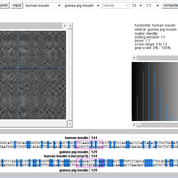
\includegraphics{/Users/muse_om92/Documents/Masterbioinfo/M1S2/BigProjet/image3.png}
Figure1: 
\end{figure}
\begin{figure}[!h]
\centering
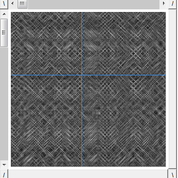
\includegraphics{/Users/muse_om92/Documents/Masterbioinfo/M1S2/BigProjet/image4.png}
Figure2:
\end{figure}
\begin{figure}[!h]
\centering
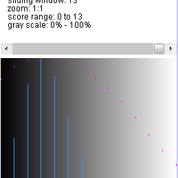
\includegraphics{/Users/muse_om92/Documents/Masterbioinfo/M1S2/BigProjet/image5.png}
Figure3:
\end{figure}
\begin{figure}[!h]
\centering
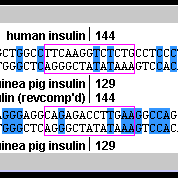
\includegraphics{/Users/muse_om92/Documents/Masterbioinfo/M1S2/BigProjet/image1.png}
Figure4:
\end{figure}

La souris a aussi son importance. En effet, en cliquant sur le graphique, s'affiche l'alignement en dessous et à droite du graphe l'histogramme (je vous laisse l'expliquer^^).\\
L'histogramme blablablabla...


\chapter{Exigences}
\section{Besoins fonctionnels}
Mathieu
version 1 : interface, liste matrice, gestion constraste/luminosité, etc : fonctionnalités demandés par le prof.

\section{Besoins non fonctionnels}
Quentin


\subsection{Fonctionnalités de la version 1.5}
Certaines fonctionnalités qui ne sont pas essentielles au bon déroulement de l'application ont été implémentée avec la version 1.5 du logiciel. Il s'agit de l'ajout d'un bouton permettant d'imprimer directement, qui pourra être remplacé par la possibilité de récupérer l'image. Les autres ajouts permettent, en combinant une action de la souris et une touche de clavier sélectionner zones d'intérêt dans l'image. Cela peut être une diagonale contenue dans la zone sélectionné si au moins la moitié des valeurs des points de cette diagonale dépassent un certain seuil (défini par l'utilisateur). Les séquences de ces diagonales peuvent ensuite être récupérées. C'est également le cas pour une autre fonctionnalité : l'utilisateur peut, en cliquant sur un point, récupérer la séquence de la diagonale sur laquelle il a cliqué, tant que les valeurs de cette diagonale sont au dessus du seuil qu'il a défini. Cette action peut être répétées, les séquences s'ajoutent. Enfin, le dernier ajout permet de voir facilement le positionnement dans les séquences avec un simple survol de la zone d'intérêt.

\subsection{Amélioration de certains points}
Quelques aspects de l'application Dotlet ne sont pas très satisfaisants et pourraient être améliorés pour donner plus de confort à l'utilisateur. Le zoom notamment, la façon de faire est peu intuitive, et il serait préférable d'utiliser la molette de la souris. L'autre point important est la gestion de la traduction : en effet, on peut choisir de comparer une séquence nucléotidique a une séquence protéique, mais en raison des multiples cadres de lectures, le calcul repose sur une moyenne avec une seuil adapté. Une solution pourrait être de ne s'occuper que de la séquence protéique la plus longue des trois cadres de lectures. En effet, la séquence la plus longue disponible est probablement la séquence d'intérêt. Enfin, l'interface pourrait gagner en esthétisme et surtout et ergonomisme.

\section{Test du programme}

30 mars, L3 ?
Jeu de données

\chapter{Environnement de Programmation}

Dans le cadre de ce projet, plusieurs langages seront utilisés. Les langages HTML/CSS serviront à structurer l'affichage dans les navigateurs web. L'interface WebGL améliorera l'affichage sur l'écran. Contrairement aux auteurs du dotlet, le développement du dot-plot sera codé en JavaScript.  Ce dernier langage est nécessaire pour utiliser WebGL.


\chapter{Architecture}
Utilisation des langages
Maquette ?

Aurélien


\chapter{Planning previsionnel}
almost done



\addcontentsline{toc}{chapter}{Conclusion}
\chapter*{Conclusion et perspectives}


\addcontentsline{toc}{chapter}{Références}
\chapter*{Références}
Le site du dotlet: http://myhits.isb-sib.ch/cgi-bin/dotlet\\
L'article des auteurs du dotlet, Thomas Junier et Marco Pagni: http://bioinformatics.oxfordjournals.org/content/16/2/178.long\\



\end{document}
